\clearpage
\setcounter{table}{0}\setcounter{figure}{0}
\renewcommand{\tablename}{Extended Data Table}
\renewcommand{\figurename}{Extended Data Fig.}

\begin{figure*}[p]
\centering
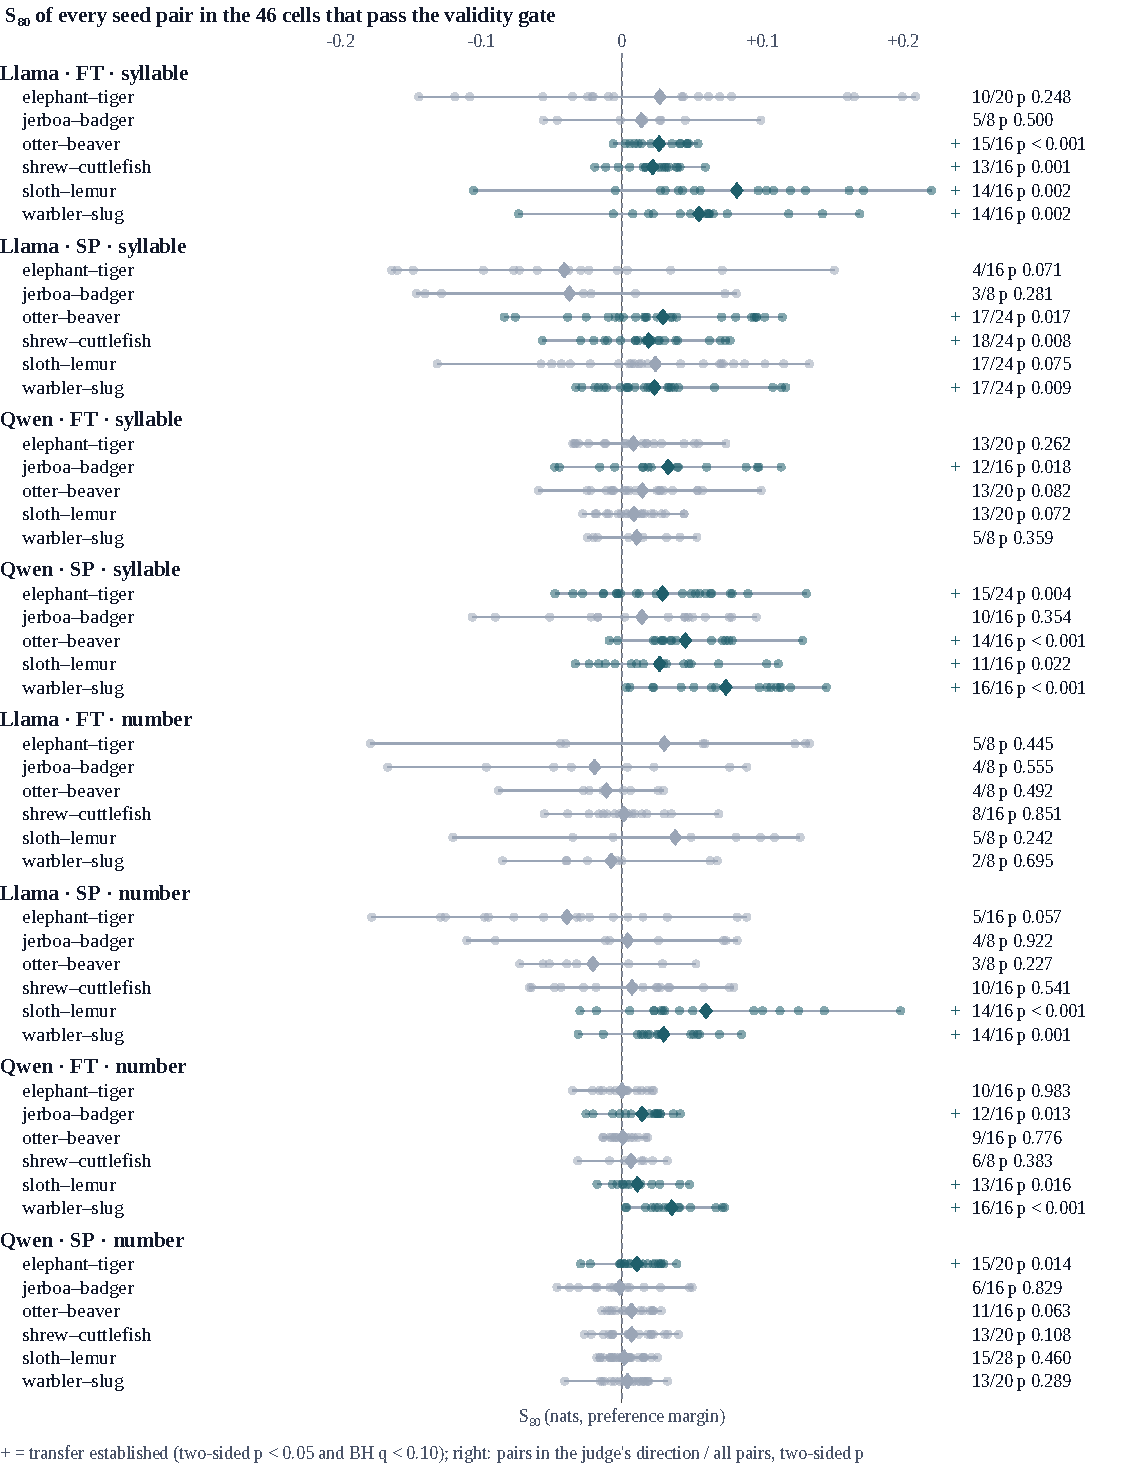
\includegraphics[height=0.86\textheight]{figs/f2.pdf}
\caption{\textbf{Every seed pair of every cell.} $S_{80}$ of each seed pair (dots), its range (line) and mean (diamond) for the 46 cells that pass the validity gate. One seed pair (\st{Llama}{FT}{syllable}{sloth--lemur}, $+0.279$) lies beyond the axis range of $\pm0.22$ and is drawn at its limit.}
\label{fig:ed-pairs}
\end{figure*}

\begin{figure*}[p]
\centering
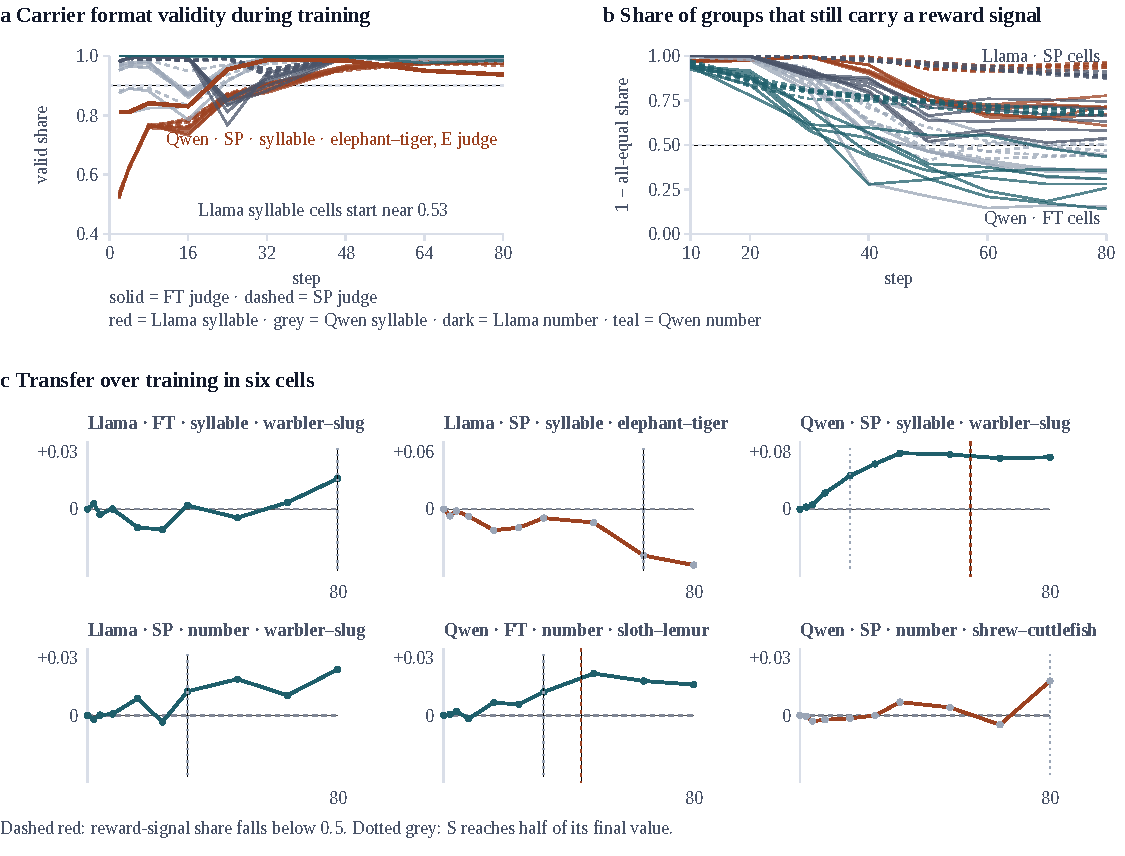
\includegraphics[width=\textwidth]{figs/f4.pdf}
\caption{\textbf{The state of the optimization, and when transfer accrues.} \textbf{a}, Carrier validity by step. \textbf{b}, Share of groups whose eight completions do not all receive the same reward. \textbf{c}, $S$ over training in six cells.}
\label{fig:dynamics}
\end{figure*}

\begin{table*}[p]
\caption{\textbf{Each judge condition's movement.} Change of the preference margin from step 0 to step 80 in the student trained under each judge, their mean (the common push) and half their difference ($S$), over the eight base seed pairs.}
\label{tab:ed-pole}
{\tabsize\setlength{\tabcolsep}{3pt}\begin{tabularx}{\textwidth}{@{}>{\raggedright\arraybackslash}p{0.16\textwidth}>{\raggedleft\arraybackslash}X>{\raggedleft\arraybackslash}X>{\raggedleft\arraybackslash}X>{\raggedleft\arraybackslash}X>{\raggedleft\arraybackslash}X@{}}
\toprule
\textbf{Cell} & \textbf{$\Delta B$, T-trained} & \textbf{$\Delta B$, E-trained} & \textbf{Common push} & \textbf{$S$ (eight pairs)} & \textbf{Pairs moving the same way}\\
\midrule
\addlinespace[2pt]\multicolumn{6}{@{}l}{\textit{Llama \textperiodcentered{} FT \textperiodcentered{} syllable}}\\
\hspace{0.6em}elephant--tiger & +0.1421 & +0.1436 & +0.1428 & $-$0.0008 & 8/8\\
\hspace{0.6em}jerboa--badger & $-$0.1820 & $-$0.2098 & $-$0.1959 & +0.0139 & 8/8\\
\hspace{0.6em}otter--beaver & $-$0.0957 & $-$0.1387 & $-$0.1172 & +0.0215 & 8/8\\
\hspace{0.6em}shrew--cuttlefish & +0.2164 & +0.1593 & +0.1879 & +0.0285 & 8/8\\
\hspace{0.6em}sloth--lemur & +0.0503 & $-$0.0965 & $-$0.0231 & +0.0734 & 4/8\\
\hspace{0.6em}warbler--slug & +0.0008 & $-$0.0354 & $-$0.0173 & +0.0181 & 6/8\\
\addlinespace[2pt]\multicolumn{6}{@{}l}{\textit{Llama \textperiodcentered{} SP \textperiodcentered{} syllable}}\\
\hspace{0.6em}elephant--tiger & $-$0.0450 & +0.0700 & +0.0125 & $-$0.0575 & 6/8\\
\hspace{0.6em}jerboa--badger & $-$0.1251 & $-$0.0504 & $-$0.0878 & $-$0.0373 & 3/8\\
\hspace{0.6em}otter--beaver & +0.0354 & $-$0.0214 & +0.0070 & +0.0284 & 5/8\\
\hspace{0.6em}shrew--cuttlefish & +0.0041 & $-$0.0319 & $-$0.0139 & +0.0180 & 7/8\\
\hspace{0.6em}sloth--lemur & $-$0.0029 & $-$0.0661 & $-$0.0345 & +0.0316 & 5/8\\
\hspace{0.6em}warbler--slug & $-$0.1314 & $-$0.1798 & $-$0.1556 & +0.0242 & 8/8\\
\addlinespace[2pt]\multicolumn{6}{@{}l}{\textit{Qwen \textperiodcentered{} FT \textperiodcentered{} syllable}}\\
\hspace{0.6em}elephant--tiger & +0.2530 & +0.2445 & +0.2487 & +0.0042 & 8/8\\
\hspace{0.6em}jerboa--badger & +0.0097 & $-$0.0071 & +0.0013 & +0.0084 & 7/8\\
\hspace{0.6em}otter--beaver & $-$0.1291 & $-$0.2046 & $-$0.1669 & +0.0377 & 8/8\\
\hspace{0.6em}sloth--lemur & $-$0.0294 & $-$0.0235 & $-$0.0264 & $-$0.0029 & 7/8\\
\hspace{0.6em}warbler--slug & $-$0.1194 & $-$0.1405 & $-$0.1299 & +0.0106 & 8/8\\
\addlinespace[2pt]\multicolumn{6}{@{}l}{\textit{Qwen \textperiodcentered{} SP \textperiodcentered{} syllable}}\\
\hspace{0.6em}elephant--tiger & +0.3117 & +0.2631 & +0.2874 & +0.0243 & 8/8\\
\hspace{0.6em}jerboa--badger & +0.0247 & $-$0.0480 & $-$0.0116 & +0.0364 & 6/8\\
\hspace{0.6em}otter--beaver & +0.0750 & $-$0.0016 & +0.0367 & +0.0383 & 5/8\\
\hspace{0.6em}sloth--lemur & $-$0.0463 & $-$0.1081 & $-$0.0772 & +0.0309 & 5/8\\
\hspace{0.6em}warbler--slug & +0.1089 & $-$0.0276 & +0.0406 & +0.0683 & 3/8\\
\addlinespace[2pt]\multicolumn{6}{@{}l}{\textit{Llama \textperiodcentered{} FT \textperiodcentered{} number}}\\
\hspace{0.6em}elephant--tiger & +0.2924 & +0.2321 & +0.2623 & +0.0302 & 7/8\\
\hspace{0.6em}jerboa--badger & +0.1323 & +0.1710 & +0.1517 & $-$0.0194 & 6/8\\
\hspace{0.6em}otter--beaver & $-$0.0444 & $-$0.0222 & $-$0.0333 & $-$0.0111 & 6/8\\
\hspace{0.6em}shrew--cuttlefish & +0.0213 & +0.0337 & +0.0275 & $-$0.0062 & 4/8\\
\hspace{0.6em}sloth--lemur & $-$0.0299 & $-$0.1057 & $-$0.0678 & +0.0379 & 5/8\\
\hspace{0.6em}warbler--slug & $-$0.3404 & $-$0.3252 & $-$0.3328 & $-$0.0076 & 8/8\\
\addlinespace[2pt]\multicolumn{6}{@{}l}{\textit{Llama \textperiodcentered{} SP \textperiodcentered{} number}}\\
\hspace{0.6em}elephant--tiger & +0.7890 & +0.8750 & +0.8320 & $-$0.0430 & 8/8\\
\hspace{0.6em}jerboa--badger & +0.8440 & +0.8357 & +0.8399 & +0.0042 & 8/8\\
\hspace{0.6em}otter--beaver & +0.4573 & +0.4986 & +0.4779 & $-$0.0206 & 8/8\\
\hspace{0.6em}shrew--cuttlefish & +0.4695 & +0.4680 & +0.4687 & +0.0008 & 8/8\\
\hspace{0.6em}sloth--lemur & $-$0.5945 & $-$0.7718 & $-$0.6832 & +0.0887 & 8/8\\
\hspace{0.6em}warbler--slug & $-$0.2020 & $-$0.2567 & $-$0.2294 & +0.0273 & 8/8\\
\addlinespace[2pt]\multicolumn{6}{@{}l}{\textit{Qwen \textperiodcentered{} FT \textperiodcentered{} number}}\\
\hspace{0.6em}elephant--tiger & +0.0206 & +0.0069 & +0.0138 & +0.0069 & 5/8\\
\hspace{0.6em}jerboa--badger & +0.0851 & +0.0571 & +0.0711 & +0.0140 & 8/8\\
\hspace{0.6em}otter--beaver & $-$0.1021 & $-$0.1082 & $-$0.1051 & +0.0030 & 8/8\\
\hspace{0.6em}shrew--cuttlefish & +0.0062 & $-$0.0068 & $-$0.0003 & +0.0065 & 6/8\\
\hspace{0.6em}sloth--lemur & $-$0.0275 & $-$0.0642 & $-$0.0459 & +0.0183 & 8/8\\
\hspace{0.6em}warbler--slug & +0.0488 & $-$0.0339 & +0.0074 & +0.0413 & 1/8\\
\addlinespace[2pt]\multicolumn{6}{@{}l}{\textit{Qwen \textperiodcentered{} SP \textperiodcentered{} number}}\\
\hspace{0.6em}elephant--tiger & +0.1327 & +0.1155 & +0.1241 & +0.0086 & 8/8\\
\hspace{0.6em}jerboa--badger & $-$0.0420 & $-$0.0276 & $-$0.0348 & $-$0.0072 & 5/8\\
\hspace{0.6em}otter--beaver & +0.0739 & +0.0522 & +0.0630 & +0.0108 & 8/8\\
\hspace{0.6em}shrew--cuttlefish & +0.1667 & +0.1257 & +0.1462 & +0.0205 & 8/8\\
\hspace{0.6em}sloth--lemur & $-$0.0756 & $-$0.0895 & $-$0.0825 & +0.0069 & 8/8\\
\hspace{0.6em}warbler--slug & $-$0.0189 & $-$0.0312 & $-$0.0251 & +0.0061 & 6/8\\
\bottomrule
\end{tabularx}
}
\end{table*}

\begin{table*}[p]
\caption{\textbf{Transfer on a cell's further seed pairs, and the combination of the two groups.}}
\label{tab:ed-further}
{\tabsize\setlength{\tabcolsep}{3pt}\begin{tabularx}{\textwidth}{@{}>{\raggedright\arraybackslash}p{0.12\textwidth}>{\raggedleft\arraybackslash}X>{\raggedleft\arraybackslash}X>{\raggedleft\arraybackslash}X>{\raggedleft\arraybackslash}p{0.115\textwidth}>{\raggedleft\arraybackslash}X>{\raggedleft\arraybackslash}X>{\raggedleft\arraybackslash}X>{\centering\arraybackslash}X>{\raggedleft\arraybackslash}X>{\raggedleft\arraybackslash}X>{\raggedleft\arraybackslash}X>{\centering\arraybackslash}X@{}}
\toprule
& \multicolumn{8}{c}{\textbf{Further seed pairs alone}} & \multicolumn{4}{c}{\textbf{All seed pairs combined}}\\
\cmidrule(lr){2-9}\cmidrule(l){10-13}
\textbf{Cell} & \textbf{Pairs} & \textbf{Further pairs} & \textbf{$S_{80}$} & \textbf{95\% CI} & \textbf{Judge's direction} & \textbf{$p$} & \textbf{$q$ (35 cells)} & \textbf{Meets criterion} & \textbf{$p$, base eight} & \textbf{Combined $p$} & \textbf{$q$ (46 cells)} & \textbf{Meets criterion}\\
\midrule
\addlinespace[3pt]\rowcolor{black!7}\multicolumn{13}{@{}l}{\textbf{FT route --- fine-tuned judges}}\\
\addlinespace[2pt]\multicolumn{13}{@{}l}{\textit{syllable \textperiodcentered{} Llama}}\\
\hspace{0.6em}elephant--tiger & 20 & 12 & +0.046 & [$-$0.018, +0.109] & 6/12 & 0.207 & 0.361 & --- & 0.977 & 0.419 & 0.642 & ---\\
\hspace{0.6em}jerboa--badger & 8 & --- & --- & --- & --- & --- & --- & --- & 0.500 & 1.000 & 1.000 & ---\\
\rowcolor{stpos!9}\hspace{0.6em}otter--beaver & 16 & 8 & +0.031 & [+0.019, +0.043] & 8/8 & 0.008 & 0.055 & yes & 0.023 & 0.001 & 0.015 & yes\\
\rowcolor{stpos!9}\hspace{0.6em}shrew--cuttlefish & 16 & 8 & +0.015 & [+0.001, +0.028] & 6/8 & 0.086 & 0.188 & --- & 0.016 & 0.006 & 0.035 & yes\\
\rowcolor{stpos!9}\hspace{0.6em}sloth--lemur & 16 & 8 & +0.090 & [+0.055, +0.128] & 8/8 & 0.008 & 0.055 & yes & 0.102 & 0.004 & 0.031 & yes\\
\rowcolor{stpos!9}\hspace{0.6em}warbler--slug & 16 & 8 & +0.091 & [+0.063, +0.123] & 8/8 & 0.008 & 0.055 & yes & 0.281 & 0.009 & 0.048 & yes\\
\addlinespace[2pt]\multicolumn{13}{@{}l}{\textit{syllable \textperiodcentered{} Qwen}}\\
\hspace{0.6em}elephant--tiger & 20 & 12 & +0.011 & [$-$0.008, +0.030] & 8/12 & 0.309 & 0.476 & --- & 0.680 & 0.414 & 0.642 & ---\\
\rowcolor{stpos!9}\hspace{0.6em}jerboa--badger & 16 & 8 & +0.057 & [+0.027, +0.087] & 7/8 & 0.016 & 0.062 & yes & 0.539 & 0.030 & 0.086 & yes\\
\hspace{0.6em}otter--beaver & 20 & 12 & $-$0.001 & [$-$0.016, +0.013] & 6/12 & 0.888 & 0.888 & --- & 0.031 & 0.100 & 0.200 & ---\\
\hspace{0.6em}sloth--lemur & 20 & 12 & +0.016 & [+0.005, +0.027] & 9/12 & 0.018 & 0.062 & yes & 0.625 & 0.074 & 0.155 & ---\\
\hspace{0.6em}warbler--slug & 8 & --- & --- & --- & --- & --- & --- & --- & 0.359 & 0.976 & 1.000 & ---\\
\addlinespace[2pt]\multicolumn{13}{@{}l}{\textit{number \textperiodcentered{} Llama}}\\
\hspace{0.6em}elephant--tiger & 8 & --- & --- & --- & --- & --- & --- & --- & 0.445 & 1.000 & 1.000 & ---\\
\hspace{0.6em}jerboa--badger & 8 & --- & --- & --- & --- & --- & --- & --- & 0.555 & 1.000 & 1.000 & ---\\
\hspace{0.6em}otter--beaver & 8 & --- & --- & --- & --- & --- & --- & --- & 0.492 & 1.000 & 1.000 & ---\\
\hspace{0.6em}shrew--cuttlefish & 16 & 8 & +0.009 & [$-$0.014, +0.032] & 5/8 & 0.492 & 0.663 & --- & 0.438 & 0.927 & 1.000 & ---\\
\hspace{0.6em}sloth--lemur & 8 & --- & --- & --- & --- & --- & --- & --- & 0.242 & 0.753 & 1.000 & ---\\
\hspace{0.6em}warbler--slug & 8 & --- & --- & --- & --- & --- & --- & --- & 0.695 & 1.000 & 1.000 & ---\\
\addlinespace[2pt]\multicolumn{13}{@{}l}{\textit{number \textperiodcentered{} Qwen}}\\
\hspace{0.6em}elephant--tiger & 16 & 8 & $-$0.007 & [$-$0.018, +0.004] & 4/8 & 0.312 & 0.476 & --- & 0.180 & 0.545 & 0.808 & ---\\
\rowcolor{stpos!9}\hspace{0.6em}jerboa--badger & 16 & 8 & +0.015 & [$-$0.001, +0.029] & 5/8 & 0.148 & 0.306 & --- & 0.047 & 0.026 & 0.086 & yes\\
\hspace{0.6em}otter--beaver & 16 & 8 & $-$0.002 & [$-$0.008, +0.005] & 4/8 & 0.648 & 0.732 & --- & 0.430 & 0.854 & 1.000 & ---\\
\hspace{0.6em}shrew--cuttlefish & 8 & --- & --- & --- & --- & --- & --- & --- & 0.383 & 1.000 & 1.000 & ---\\
\rowcolor{stpos!9}\hspace{0.6em}sloth--lemur & 16 & 8 & +0.004 & [$-$0.001, +0.008] & 6/8 & 0.164 & 0.317 & --- & 0.055 & 0.032 & 0.086 & yes\\
\rowcolor{stpos!9}\hspace{0.6em}warbler--slug & 16 & 8 & +0.030 & [+0.016, +0.044] & 8/8 & 0.008 & 0.055 & yes & 0.008 & $<$0.001 & 0.008 & yes\\
\addlinespace[3pt]\rowcolor{black!7}\multicolumn{13}{@{}l}{\textbf{SP route --- persona judges}}\\
\addlinespace[2pt]\multicolumn{13}{@{}l}{\textit{syllable \textperiodcentered{} Llama}}\\
\rowcolor{stpos!9}\hspace{0.6em}elephant--tiger & 16 & 8 & $-$0.024 & [$-$0.093, +0.047] & 3/8 & 0.531 & 0.689 & --- & 0.016 & 0.030 & 0.086 & yes\\
\hspace{0.6em}jerboa--badger & 8 & --- & --- & --- & --- & --- & --- & --- & 0.281 & 0.833 & 1.000 & ---\\
\rowcolor{stpos!9}\hspace{0.6em}otter--beaver & 24 & 16 & +0.030 & [+0.002, +0.056] & 12/16 & 0.061 & 0.143 & --- & 0.195 & 0.041 & 0.099 & yes\\
\rowcolor{stpos!9}\hspace{0.6em}shrew--cuttlefish & 24 & 16 & +0.020 & [+0.005, +0.035] & 12/16 & 0.023 & 0.073 & yes & 0.211 & 0.019 & 0.078 & yes\\
\hspace{0.6em}sloth--lemur & 24 & 16 & +0.020 & [$-$0.011, +0.049] & 11/16 & 0.217 & 0.362 & --- & 0.211 & 0.125 & 0.231 & ---\\
\rowcolor{stpos!9}\hspace{0.6em}warbler--slug & 24 & 16 & +0.023 & [+0.004, +0.044] & 12/16 & 0.041 & 0.118 & --- & 0.141 & 0.022 & 0.084 & yes\\
\addlinespace[2pt]\multicolumn{13}{@{}l}{\textit{syllable \textperiodcentered{} Qwen}}\\
\rowcolor{stpos!9}\hspace{0.6em}elephant--tiger & 24 & 16 & +0.031 & [+0.010, +0.054] & 10/16 & 0.016 & 0.062 & yes & 0.156 & 0.011 & 0.049 & yes\\
\hspace{0.6em}jerboa--badger & 16 & 8 & $-$0.008 & [$-$0.054, +0.038] & 4/8 & 0.742 & 0.787 & --- & 0.039 & 0.133 & 0.236 & ---\\
\rowcolor{stpos!9}\hspace{0.6em}otter--beaver & 16 & 8 & +0.052 & [+0.026, +0.080] & 7/8 & 0.016 & 0.062 & yes & 0.016 & 0.001 & 0.015 & yes\\
\hspace{0.6em}sloth--lemur & 16 & 8 & +0.023 & [$-$0.001, +0.052] & 5/8 & 0.172 & 0.317 & --- & 0.109 & 0.060 & 0.131 & ---\\
\rowcolor{stpos!9}\hspace{0.6em}warbler--slug & 16 & 8 & +0.080 & [+0.053, +0.107] & 8/8 & 0.008 & 0.055 & yes & 0.008 & $<$0.001 & 0.008 & yes\\
\addlinespace[2pt]\multicolumn{13}{@{}l}{\textit{number \textperiodcentered{} Llama}}\\
\hspace{0.6em}elephant--tiger & 16 & 8 & $-$0.035 & [$-$0.101, +0.030] & 3/8 & 0.344 & 0.501 & --- & 0.047 & 0.052 & 0.121 & ---\\
\hspace{0.6em}jerboa--badger & 8 & --- & --- & --- & --- & --- & --- & --- & 0.922 & 1.000 & 1.000 & ---\\
\hspace{0.6em}otter--beaver & 8 & --- & --- & --- & --- & --- & --- & --- & 0.227 & 0.720 & 1.000 & ---\\
\hspace{0.6em}shrew--cuttlefish & 16 & 8 & +0.014 & [$-$0.017, +0.043] & 5/8 & 0.438 & 0.613 & --- & 0.961 & 0.684 & 0.983 & ---\\
\rowcolor{stpos!9}\hspace{0.6em}sloth--lemur & 16 & 8 & +0.031 & [+0.007, +0.056] & 7/8 & 0.055 & 0.137 & --- & 0.016 & 0.004 & 0.031 & yes\\
\rowcolor{stpos!9}\hspace{0.6em}warbler--slug & 16 & 8 & +0.032 & [+0.015, +0.049] & 7/8 & 0.016 & 0.062 & yes & 0.070 & 0.005 & 0.033 & yes\\
\addlinespace[2pt]\multicolumn{13}{@{}l}{\textit{number \textperiodcentered{} Qwen}}\\
\rowcolor{stpos!9}\hspace{0.6em}elephant--tiger & 20 & 12 & +0.012 & [+0.002, +0.021] & 10/12 & 0.044 & 0.118 & --- & 0.203 & 0.032 & 0.086 & yes\\
\hspace{0.6em}jerboa--badger & 16 & 8 & +0.004 & [$-$0.012, +0.022] & 4/8 & 0.680 & 0.743 & --- & 0.477 & 0.900 & 1.000 & ---\\
\hspace{0.6em}otter--beaver & 16 & 8 & +0.003 & [$-$0.005, +0.012] & 5/8 & 0.586 & 0.726 & --- & 0.062 & 0.104 & 0.200 & ---\\
\rowcolor{stpos!9}\hspace{0.6em}shrew--cuttlefish & 20 & 12 & $-$0.002 & [$-$0.010, +0.006] & 5/12 & 0.613 & 0.726 & --- & 0.008 & 0.037 & 0.096 & yes\\
\hspace{0.6em}sloth--lemur & 28 & 20 & $-$0.001 & [$-$0.005, +0.004] & 9/20 & 0.832 & 0.857 & --- & 0.148 & 0.358 & 0.610 & ---\\
\hspace{0.6em}warbler--slug & 20 & 12 & +0.003 & [$-$0.008, +0.011] & 9/12 & 0.623 & 0.726 & --- & 0.320 & 0.399 & 0.642 & ---\\
\bottomrule
\end{tabularx}
}
\end{table*}

\begin{table*}[p]
\caption{\textbf{Carrier channel decomposition, one row per cell.} Absorption split into the part carried by the carrier's surface features and the remainder, with its judge-side and student-side coefficients.}
\label{tab:ed-chan}
{\tabsize\setlength{\tabcolsep}{3pt}\begin{tabularx}{\textwidth}{@{}>{\raggedright\arraybackslash}p{0.13\textwidth}>{\raggedleft\arraybackslash}X>{\raggedleft\arraybackslash}X>{\raggedleft\arraybackslash}X>{\raggedleft\arraybackslash}X>{\raggedleft\arraybackslash}X>{\raggedleft\arraybackslash}X>{\raggedleft\arraybackslash}X@{}}
\toprule
\textbf{Cell} & \textbf{Absorption (training instance)} & \textbf{Feature part} & \textbf{Residual} & \textbf{Judge-side coefficient} & \textbf{Student-side coefficient} & \textbf{Instance-mean absorption} & \textbf{Its feature part}\\
\midrule
\addlinespace[3pt]\rowcolor{black!7}\multicolumn{8}{@{}l}{\textbf{FT route --- fine-tuned judges}}\\
\addlinespace[2pt]\multicolumn{8}{@{}l}{\textit{syllable \textperiodcentered{} Llama letters + bigrams; coefficient = match with the animal-name letters}}\\
\hspace{0.6em}elephant--tiger & +0.245 & +0.115 & +0.130 & +0.539 & +0.417 & +0.150 & +0.102\\
\hspace{0.6em}jerboa--badger & +0.199 & +0.082 & +0.117 & +0.374 & +0.540 & +0.070 & +0.039\\
\hspace{0.6em}otter--beaver & +0.180 & +0.073 & +0.107 & +0.297 & +0.685 & +0.261 & +0.115\\
\hspace{0.6em}shrew--cuttlefish & +0.209 & +0.084 & +0.125 & $-$0.068 & +0.471 & +0.163 & +0.085\\
\hspace{0.6em}sloth--lemur & +0.065 & +0.060 & +0.005 & +0.438 & +0.464 & +0.228 & +0.144\\
\hspace{0.6em}warbler--slug & +0.140 & +0.072 & +0.067 & +0.366 & +0.548 & +0.243 & +0.089\\
\addlinespace[2pt]\multicolumn{8}{@{}l}{\textit{syllable \textperiodcentered{} Qwen letters + bigrams; coefficient = match with the animal-name letters}}\\
\hspace{0.6em}elephant--tiger & +0.101 & +0.078 & +0.023 & +0.223 & +0.143 & +0.143 & +0.098\\
\hspace{0.6em}jerboa--badger & +0.153 & +0.045 & +0.108 & +0.420 & +0.479 & +0.145 & +0.043\\
\hspace{0.6em}otter--beaver & +0.110 & +0.022 & +0.088 & +0.414 & +0.546 & +0.123 & +0.021\\
\hspace{0.6em}sloth--lemur & +0.044 & +0.009 & +0.036 & +0.067 & +0.204 & +0.046 & +0.002\\
\hspace{0.6em}warbler--slug & +0.076 & +0.004 & +0.072 & +0.344 & +0.331 & +0.193 & +0.079\\
\addlinespace[2pt]\multicolumn{8}{@{}l}{\textit{number \textperiodcentered{} Llama number statistics; coefficient = correlation with mean value}}\\
\hspace{0.6em}elephant--tiger & +0.225 & $-$0.027 & +0.252 & +0.099 & $-$0.081 & +0.142 & $-$0.027\\
\hspace{0.6em}jerboa--badger & +0.241 & +0.022 & +0.218 & +0.039 & $-$0.008 & $-$0.216 & +0.030\\
\hspace{0.6em}otter--beaver & +0.207 & +0.005 & +0.202 & $-$0.127 & $-$0.039 & +0.108 & +0.018\\
\hspace{0.6em}shrew--cuttlefish & +0.188 & +0.056 & +0.132 & +0.052 & +0.008 & +0.105 & +0.020\\
\hspace{0.6em}sloth--lemur & $-$0.048 & +0.016 & $-$0.064 & +0.069 & +0.051 & $-$0.036 & +0.045\\
\hspace{0.6em}warbler--slug & +0.097 & +0.003 & +0.094 & $-$0.156 & +0.085 & +0.183 & +0.013\\
\addlinespace[2pt]\multicolumn{8}{@{}l}{\textit{number \textperiodcentered{} Qwen number statistics; coefficient = correlation with mean value}}\\
\hspace{0.6em}elephant--tiger & +0.110 & +0.073 & +0.037 & $-$0.068 & $-$0.032 & +0.065 & +0.077\\
\hspace{0.6em}jerboa--badger & +0.004 & $-$0.010 & +0.014 & $-$0.215 & +0.127 & +0.052 & +0.020\\
\hspace{0.6em}otter--beaver & +0.051 & +0.004 & +0.046 & +0.148 & $-$0.026 & $-$0.017 & $-$0.035\\
\hspace{0.6em}shrew--cuttlefish & +0.013 & $-$0.047 & +0.060 & +0.208 & $-$0.314 & +0.015 & $-$0.094\\
\hspace{0.6em}sloth--lemur & $-$0.109 & $-$0.073 & $-$0.036 & $-$0.051 & +0.274 & $-$0.137 & $-$0.103\\
\hspace{0.6em}warbler--slug & +0.332 & +0.191 & +0.141 & +0.143 & +0.103 & +0.386 & +0.246\\
\addlinespace[3pt]\rowcolor{black!7}\multicolumn{8}{@{}l}{\textbf{SP route --- persona judges}}\\
\addlinespace[2pt]\multicolumn{8}{@{}l}{\textit{syllable \textperiodcentered{} Llama letters + bigrams; coefficient = match with the animal-name letters}}\\
\hspace{0.6em}elephant--tiger & $-$0.051 & +0.044 & $-$0.095 & +0.394 & +0.331 & +0.024 & +0.077\\
\hspace{0.6em}jerboa--badger & $-$0.072 & +0.017 & $-$0.089 & +0.579 & +0.531 & $-$0.071 & +0.009\\
\hspace{0.6em}otter--beaver & +0.041 & +0.094 & $-$0.052 & +0.423 & +0.622 & +0.147 & +0.129\\
\hspace{0.6em}shrew--cuttlefish & +0.094 & +0.031 & +0.063 & +0.467 & +0.590 & +0.108 & +0.051\\
\hspace{0.6em}sloth--lemur & +0.168 & +0.090 & +0.078 & +0.671 & +0.519 & +0.164 & +0.099\\
\hspace{0.6em}warbler--slug & +0.183 & +0.102 & +0.081 & +0.545 & +0.619 & +0.181 & +0.106\\
\addlinespace[2pt]\multicolumn{8}{@{}l}{\textit{syllable \textperiodcentered{} Qwen letters + bigrams; coefficient = match with the animal-name letters}}\\
\hspace{0.6em}elephant--tiger & +0.041 & $-$0.035 & +0.076 & +0.409 & +0.095 & +0.053 & $-$0.035\\
\hspace{0.6em}jerboa--badger & +0.184 & +0.056 & +0.128 & +0.342 & +0.498 & +0.159 & +0.052\\
\hspace{0.6em}otter--beaver & +0.173 & +0.080 & +0.093 & +0.111 & +0.487 & +0.195 & +0.100\\
\hspace{0.6em}sloth--lemur & +0.085 & $-$0.007 & +0.092 & +0.380 & +0.258 & +0.093 & $-$0.000\\
\hspace{0.6em}warbler--slug & +0.333 & +0.166 & +0.167 & +0.336 & +0.323 & +0.317 & +0.154\\
\addlinespace[2pt]\multicolumn{8}{@{}l}{\textit{number \textperiodcentered{} Llama number statistics; coefficient = correlation with mean value}}\\
\hspace{0.6em}elephant--tiger & $-$0.416 & $-$0.030 & $-$0.385 & $-$0.006 & $-$0.044 & $-$0.488 & $-$0.024\\
\hspace{0.6em}jerboa--badger & $-$0.349 & $-$0.023 & $-$0.326 & $-$0.055 & $-$0.010 & $-$0.398 & $-$0.030\\
\hspace{0.6em}otter--beaver & $-$0.465 & $-$0.016 & $-$0.449 & $-$0.059 & $-$0.049 & $-$0.246 & $-$0.009\\
\hspace{0.6em}shrew--cuttlefish & +0.415 & +0.012 & +0.403 & +0.031 & +0.045 & +0.310 & +0.024\\
\hspace{0.6em}sloth--lemur & +0.218 & $-$0.013 & +0.231 & $-$0.088 & +0.059 & +0.081 & $-$0.026\\
\hspace{0.6em}warbler--slug & +0.033 & +0.043 & $-$0.010 & +0.066 & +0.009 & $-$0.031 & +0.039\\
\addlinespace[2pt]\multicolumn{8}{@{}l}{\textit{number \textperiodcentered{} Qwen number statistics; coefficient = correlation with mean value}}\\
\hspace{0.6em}elephant--tiger & +0.046 & +0.045 & +0.001 & $-$0.024 & $-$0.012 & +0.047 & +0.070\\
\hspace{0.6em}jerboa--badger & +0.093 & +0.093 & $-$0.000 & +0.107 & +0.079 & +0.217 & +0.139\\
\hspace{0.6em}otter--beaver & +0.133 & +0.043 & +0.090 & $-$0.050 & $-$0.048 & +0.184 & +0.052\\
\hspace{0.6em}shrew--cuttlefish & +0.066 & +0.057 & +0.009 & $-$0.038 & $-$0.283 & +0.136 & +0.110\\
\hspace{0.6em}sloth--lemur & $-$0.129 & $-$0.070 & $-$0.059 & $-$0.071 & +0.247 & $-$0.180 & $-$0.117\\
\hspace{0.6em}warbler--slug & +0.180 & +0.104 & +0.076 & +0.055 & +0.163 & +0.198 & +0.107\\
\bottomrule
\end{tabularx}
}
\end{table*}

\begin{table*}[p]
\caption{\textbf{Reward intervention.} Training on $c + \alpha s$, where $c$ is the part of the reward shared by the two judges and $s$ the between-judge part; eight seed pairs per condition. Dashes mark the $\alpha = 1$ reference and values not logged for that run.}
\label{tab:ed-alpha}
{\tabsize\begin{tabularx}{\textwidth}{@{}>{\raggedright\arraybackslash}p{0.24\textwidth}c>{\raggedleft\arraybackslash}X>{\raggedleft\arraybackslash}X>{\raggedleft\arraybackslash}X>{\raggedleft\arraybackslash}X@{}}
\toprule
\textbf{Cell} & $\boldsymbol{\alpha}$ & $\boldsymbol{S_{80}}$ \textbf{(pairs in judge's direction)} & \textbf{Paired difference from} $\boldsymbol{\alpha=1}$ & \textbf{KL} & \textbf{Validity} \\
\midrule
\st{Llama}{FT}{syllable}{sloth--lemur} & 0 & $-0.034$ (2/8) & $-0.107$, $p=0.023$ & 1.04 & 0.822 \\
 & 1 & $+0.073$ & --- & 1.13 & 0.820 \\
 & 2 & $+0.118$ (8/8) & $+0.044$, $p=0.24$ & 1.06 & 0.814 \\
\midrule
\st{Llama}{SP}{number}{sloth--lemur} & 0 & $+0.004$ (5/8) & $-0.084$, $p=0.031$ & 0.89 & 0.987 \\
 & 1 & $+0.089$ & --- & 0.92 & 0.987 \\
 & 2 & $+0.045$ & $-0.044$, $p=0.13$ & --- & --- \\
\bottomrule
\end{tabularx}
}
\end{table*}

\begin{table*}[p]
\caption{\textbf{The state of training, one row per cell.} Carrier validity, the share of groups that carry a reward signal, and when transfer accrues.}
\label{tab:ed-time}
{\tabsize\setlength{\tabcolsep}{3pt}\begin{tabularx}{\textwidth}{@{}>{\raggedright\arraybackslash}p{0.13\textwidth}>{\raggedleft\arraybackslash}X>{\raggedleft\arraybackslash}X>{\raggedleft\arraybackslash}X>{\raggedleft\arraybackslash}X>{\raggedleft\arraybackslash}X@{}}
\toprule
\textbf{Cell} & \textbf{Validity, step 2 / 48 / 80} & \textbf{Lowest run, step 80} & \textbf{Reward-signal share, step 10 / 40 / 80} & \textbf{First step with signal share $<0.5$} & \textbf{Step reaching 50\% / 80\% of $S_{80}$}\\
\midrule
\addlinespace[3pt]\rowcolor{black!7}\multicolumn{6}{@{}l}{\textbf{FT route --- fine-tuned judges}}\\
\addlinespace[2pt]\multicolumn{6}{@{}l}{\textit{syllable \textperiodcentered{} Llama}}\\
\hspace{0.6em}elephant--tiger & 0.530 / 0.961 / 0.981 & 0.973 & 0.97 / 0.92 / 0.61 & never & ---\\
\hspace{0.6em}jerboa--badger & 0.523 / 0.958 / 0.980 & 0.964 & 0.97 / 0.91 / 0.78 & never & ---\\
\hspace{0.6em}otter--beaver & 0.542 / 0.967 / 0.980 & 0.968 & 0.97 / 0.90 / 0.72 & never & 64 / 64\\
\hspace{0.6em}shrew--cuttlefish & 0.526 / 0.959 / 0.981 & 0.971 & 0.97 / 0.95 / 0.71 & never & 32 / 48\\
\hspace{0.6em}sloth--lemur & 0.525 / 0.965 / 0.984 & 0.972 & 0.97 / 0.91 / 0.67 & never & 48 / 48\\
\hspace{0.6em}warbler--slug & 0.535 / 0.962 / 0.980 & 0.967 & 0.98 / 0.95 / 0.71 & never & 80 / 80\\
\addlinespace[2pt]\multicolumn{6}{@{}l}{\textit{syllable \textperiodcentered{} Qwen}}\\
\hspace{0.6em}elephant--tiger & 0.809 / 0.996 / 0.999 & 0.998 & 1.00 / 0.28 / 0.16 & 36 & ---\\
\hspace{0.6em}jerboa--badger & 0.971 / 0.996 / 0.991 & 0.953 & 1.00 / 0.56 / 0.31 & 46 & 8 / 8\\
\hspace{0.6em}otter--beaver & 0.965 / 0.998 / 0.997 & 0.973 & 1.00 / 0.62 / 0.35 & 48 & ---\\
\hspace{0.6em}sloth--lemur & 0.953 / 0.990 / 0.991 & 0.956 & 1.00 / 0.56 / 0.37 & 46 & ---\\
\hspace{0.6em}warbler--slug & 0.875 / 0.995 / 0.994 & 0.980 & 1.00 / 0.77 / 0.44 & 68 & ---\\
\addlinespace[2pt]\multicolumn{6}{@{}l}{\textit{number \textperiodcentered{} Llama}}\\
\hspace{0.6em}elephant--tiger & 0.980 / 0.998 / 0.998 & 0.995 & 1.00 / 0.79 / 0.54 & never & ---\\
\hspace{0.6em}jerboa--badger & 0.983 / 0.998 / 0.999 & 0.996 & 1.00 / 0.83 / 0.63 & never & ---\\
\hspace{0.6em}otter--beaver & 0.984 / 0.998 / 0.998 & 0.994 & 1.00 / 0.87 / 0.70 & never & ---\\
\hspace{0.6em}shrew--cuttlefish & 0.982 / 0.997 / 0.998 & 0.993 & 1.00 / 0.85 / 0.75 & never & ---\\
\hspace{0.6em}sloth--lemur & 0.982 / 0.997 / 0.998 & 0.994 & 1.00 / 0.88 / 0.67 & never & ---\\
\hspace{0.6em}warbler--slug & 0.985 / 0.996 / 0.998 & 0.996 & 1.00 / 0.80 / 0.58 & never & ---\\
\addlinespace[2pt]\multicolumn{6}{@{}l}{\textit{number \textperiodcentered{} Qwen}}\\
\hspace{0.6em}elephant--tiger & 1.000 / 0.999 / 0.998 & 0.974 & 0.94 / 0.60 / 0.43 & 68 & ---\\
\hspace{0.6em}jerboa--badger & 1.000 / 0.999 / 0.986 & 0.862 & 0.93 / 0.44 / 0.14 & 36 & 24 / 24\\
\hspace{0.6em}otter--beaver & 1.000 / 0.997 / 1.000 & 0.999 & 0.94 / 0.28 / 0.36 & 34 & ---\\
\hspace{0.6em}shrew--cuttlefish & 1.000 / 0.994 / 0.997 & 0.975 & 0.93 / 0.54 / 0.26 & 42 & ---\\
\hspace{0.6em}sloth--lemur & 1.000 / 0.999 / 1.000 & 0.999 & 0.94 / 0.57 / 0.31 & 44 & 32 / 48\\
\hspace{0.6em}warbler--slug & 1.000 / 0.999 / 0.997 & 0.959 & 0.95 / 0.45 / 0.28 & 38 & 24 / 24\\
\addlinespace[3pt]\rowcolor{black!7}\multicolumn{6}{@{}l}{\textbf{SP route --- persona judges}}\\
\addlinespace[2pt]\multicolumn{6}{@{}l}{\textit{syllable \textperiodcentered{} Llama}}\\
\hspace{0.6em}elephant--tiger & 0.535 / 0.954 / 0.975 & 0.962 & 0.98 / 1.00 / 0.96 & never & ---\\
\hspace{0.6em}jerboa--badger & 0.526 / 0.956 / 0.974 & 0.963 & 0.97 / 0.98 / 0.93 & never & ---\\
\hspace{0.6em}otter--beaver & 0.529 / 0.957 / 0.975 & 0.946 & 0.98 / 0.98 / 0.95 & never & 48 / 64\\
\hspace{0.6em}shrew--cuttlefish & 0.535 / 0.951 / 0.973 & 0.959 & 0.98 / 0.98 / 0.93 & never & 8 / 32\\
\hspace{0.6em}sloth--lemur & 0.530 / 0.958 / 0.975 & 0.950 & 0.97 / 0.99 / 0.95 & never & ---\\
\hspace{0.6em}warbler--slug & 0.520 / 0.957 / 0.968 & 0.941 & 0.97 / 0.99 / 0.96 & never & 24 / 24\\
\addlinespace[2pt]\multicolumn{6}{@{}l}{\textit{syllable \textperiodcentered{} Qwen}}\\
\hspace{0.6em}elephant--tiger & 0.811 / 0.985 / 0.937 & 0.746 & 0.99 / 0.55 / 0.53 & 43 & 32 / 48\\
\hspace{0.6em}jerboa--badger & 0.972 / 0.994 / 0.993 & 0.971 & 1.00 / 0.73 / 0.44 & 53 & ---\\
\hspace{0.6em}otter--beaver & 0.967 / 0.994 / 0.987 & 0.954 & 1.00 / 0.71 / 0.47 & 67 & 24 / 32\\
\hspace{0.6em}sloth--lemur & 0.952 / 0.992 / 0.986 & 0.955 & 0.99 / 0.64 / 0.45 & 49 & 32 / 64\\
\hspace{0.6em}warbler--slug & 0.883 / 0.988 / 0.981 & 0.931 & 1.00 / 0.63 / 0.50 & 54 & 16 / 24\\
\addlinespace[2pt]\multicolumn{6}{@{}l}{\textit{number \textperiodcentered{} Llama}}\\
\hspace{0.6em}elephant--tiger & 0.983 / 0.997 / 0.999 & 0.998 & 1.00 / 0.98 / 0.88 & never & ---\\
\hspace{0.6em}jerboa--badger & 0.980 / 0.997 / 0.999 & 0.998 & 1.00 / 0.97 / 0.87 & never & ---\\
\hspace{0.6em}otter--beaver & 0.980 / 0.996 / 0.998 & 0.994 & 1.00 / 0.97 / 0.89 & never & ---\\
\hspace{0.6em}shrew--cuttlefish & 0.984 / 0.996 / 0.999 & 0.998 & 1.00 / 0.98 / 0.91 & never & ---\\
\hspace{0.6em}sloth--lemur & 0.980 / 0.995 / 0.999 & 0.998 & 1.00 / 0.98 / 0.89 & never & 32 / 48\\
\hspace{0.6em}warbler--slug & 0.983 / 0.996 / 0.998 & 0.996 & 1.00 / 0.98 / 0.90 & never & 32 / 80\\
\addlinespace[2pt]\multicolumn{6}{@{}l}{\textit{number \textperiodcentered{} Qwen}}\\
\hspace{0.6em}elephant--tiger & 1.000 / 1.000 / 1.000 & 1.000 & 0.94 / 0.75 / 0.67 & never & 16 / 48\\
\hspace{0.6em}jerboa--badger & 1.000 / 1.000 / 1.000 & 1.000 & 0.96 / 0.75 / 0.67 & never & ---\\
\hspace{0.6em}otter--beaver & 1.000 / 1.000 / 1.000 & 1.000 & 0.97 / 0.78 / 0.70 & never & ---\\
\hspace{0.6em}shrew--cuttlefish & 1.000 / 1.000 / 1.000 & 1.000 & 0.97 / 0.78 / 0.68 & never & ---\\
\hspace{0.6em}sloth--lemur & 1.000 / 1.000 / 1.000 & 1.000 & 0.96 / 0.77 / 0.68 & never & ---\\
\hspace{0.6em}warbler--slug & 1.000 / 1.000 / 1.000 & 1.000 & 0.95 / 0.76 / 0.68 & never & ---\\
\bottomrule
\end{tabularx}
}
\end{table*}

\begin{table*}[p]
\caption{\textbf{Judges that are not the student's own model.} For each route and student, the main-grid judges beside the other family's 1B-class judges and 8B judges of either family, with everything else held fixed.}
\label{tab:judges}
{\tabsize\setlength{\tabcolsep}{3pt}\begin{tabularx}{\textwidth}{@{}>{\raggedright\arraybackslash}p{0.15\textwidth}>{\raggedleft\arraybackslash}X>{\raggedleft\arraybackslash}X>{\raggedleft\arraybackslash}X>{\raggedleft\arraybackslash}X>{\raggedleft\arraybackslash}X>{\raggedleft\arraybackslash}X>{\raggedleft\arraybackslash}X@{\hspace{10pt}}>{\raggedright\arraybackslash}p{0.15\textwidth}@{}}
\toprule
\textbf{Judge} & \textbf{Emission $\Lambda$ (mean)} & \textbf{$\Lambda$ lower bound $>0$} & \textbf{Trait alignment with own-model judge ($r$)} & \textbf{$|$Absorption$|$} & \textbf{Absorption sign as own model} & \textbf{Judge term} & \textbf{Absorption vs $S_{80}$ ($r$)} & \textbf{Transfer}\\
\midrule
\addlinespace[3pt]\rowcolor{black!7}\multicolumn{9}{@{}l}{\textbf{FT route --- fine-tuned judges}}\\
\addlinespace[2pt]\multicolumn{9}{@{}l}{\textit{Student Llama-3.2-1B}}\\
\hspace{0.6em}Own model (main grid) & +0.117 & 12/12 & --- & 0.170 & --- & 0.113 & +0.38 & 4 of 12 established\\
\hspace{0.6em}Other family, 1B class & +0.128 & 12/12 & +0.03 & 0.066 & 8/12 & 0.037 & $-$0.05 & none established\\
\hspace{0.6em}Same family, 8B & +0.103 & 12/12 & +0.07 & 0.090 & 9/12 & 0.072 & --- & 0 of 2 trained cells\\
\hspace{0.6em}Other family, 8B & +0.214 & 12/12 & +0.02 & 0.047 & 9/12 & 0.080 & --- & 0 of 2 trained cells\\
\addlinespace[2pt]\multicolumn{9}{@{}l}{\textit{Student Qwen3-1.7B}}\\
\hspace{0.6em}Own model (main grid) & +0.136 & 10/11 & --- & 0.100 & --- & 0.119 & +0.59 & 4 of 11 established\\
\hspace{0.6em}Other family, 1B class & +0.138 & 10/11 & +0.03 & 0.084 & 7/11 & 0.095 & +0.40 & none established\\
\hspace{0.6em}Same family, 8B & +0.223 & 11/11 & +0.01 & 0.092 & 7/11 & 0.062 & --- & 0 of 2 trained cells\\
\hspace{0.6em}Other family, 8B & +0.111 & 9/11 & +0.04 & 0.144 & 9/11 & 0.119 & --- & 0 of 2 trained cells\\
\addlinespace[3pt]\rowcolor{black!7}\multicolumn{9}{@{}l}{\textbf{SP route --- persona judges}}\\
\addlinespace[2pt]\multicolumn{9}{@{}l}{\textit{Student Llama-3.2-1B}}\\
\hspace{0.6em}Own model (main grid) & +0.231 & 12/12 & --- & 0.209 & --- & 0.209 & +0.38 & 5 of 12 established\\
\hspace{0.6em}Other family, 1B class & +0.274 & 12/12 & +0.02 & 0.040 & 7/12 & 0.028 & $-$0.05 & none established\\
\hspace{0.6em}Same family, 8B & +0.262 & 12/12 & +0.07 & 0.067 & 7/12 & 0.038 & --- & 0 of 2 trained cells\\
\hspace{0.6em}Other family, 8B & +0.253 & 12/12 & +0.06 & 0.052 & 7/12 & 0.047 & --- & 0 of 2 trained cells\\
\addlinespace[2pt]\multicolumn{9}{@{}l}{\textit{Student Qwen3-1.7B}}\\
\hspace{0.6em}Own model (main grid) & +0.366 & 11/11 & --- & 0.133 & --- & 0.080 & +0.59 & 5 of 11 established\\
\hspace{0.6em}Other family, 1B class & +0.349 & 11/11 & +0.04 & 0.093 & 5/11 & 0.094 & +0.40 & none established\\
\hspace{0.6em}Same family, 8B & +0.413 & 11/11 & +0.12 & 0.067 & 6/11 & 0.072 & --- & 0 of 2 trained cells\\
\hspace{0.6em}Other family, 8B & +0.287 & 11/11 & +0.12 & 0.130 & 10/11 & 0.090 & --- & 0 of 2 trained cells\\
\bottomrule
\end{tabularx}
}
\end{table*}
